\documentclass[a4paper,twoside,notitlepage,11pt]{article}
\usepackage{graphicx}
\usepackage{hyperref}
\usepackage{fancyeq}
\usepackage{amstext}
\usepackage{tabularx}
\usepackage{amssymb}
\usepackage{fancyhdr}
\usepackage{multirow}
\usepackage{tocloft}
\usepackage{lscape}
\usepackage{transparent}
\usepackage{subcaption}
\usepackage{rotating}
\usepackage{titletoc}
\usepackage{setspace}
\usepackage[all]{xy}
\usepackage{nccmath}
\usepackage[a4paper,hmargin=2.5cm,vmargin=2.5cm]{geometry}
\usepackage[hypcap]{caption}
\usepackage{qtree}
\usepackage{cleveref}
\usepackage{mathpartir}
\usepackage{listings}
\usepackage{multirow}
\usepackage{enumitem}
\usepackage{float}
\usepackage[compact]{titlesec}
\usepackage{layouts}
\usepackage{wrapfig}
\usepackage{listings}
\usepackage{color}
\usepackage{xcolor}
\usepackage{ulem}

\hypersetup{
    unicode=false,
    pdftoolbar=true,  
    pdfmenubar=true,     
    pdffitwindow=false,    
    pdfstartview={FitH},  
    pdftitle={Title},  
    pdfauthor={Craig Knott},
    pdfsubject={CS},
    pdfnewwindow=true,  
    colorlinks=true,  
    linkcolor=black,  
    citecolor=black, 
    filecolor=black,  
    urlcolor=black  
}

\newcommand{\paperTitleShort}{Web-based Fuzzy Logic Visualisation and Inferencing System}
\newcommand{\paperTitle}{Improving usability and accessibility of Fuzzy Logic software systems with a web-based approach}

\setlength{\parskip}{0.25em}

\renewcommand{\headrulewidth}{0.0pt}

\fancypagestyle{plain}{
	\fancyhf{}
	\fancyhead[LO]{Craig Knott}
	\fancyhead[CO]{\textit{\paperTitleShort}}
	\fancyhead[RO]{\thepage}
	\fancyhead[LE]{\thepage}
	\fancyhead[CE]{\textit{\paperTitleShort}}
	\fancyhead[RE]{Craig Knott}
}

\fancypagestyle{appendix}{
	\fancyhf{}
	\fancyhead[LO]{Craig Knott}
	\fancyhead[CO]{\textit{\paperTitleShort}}
	\fancyhead[RO]{Appendix \thepage}
	\fancyhead[LE]{Appendix \thepage}
	\fancyhead[CE]{\textit{\paperTitleShort}}
	\fancyhead[RE]{Craig Knott}
}

\fancypagestyle{biblio}{
	\fancyhf{}
	\fancyhead[LO]{cxk01u}
	\fancyhead[CO]{\textit{\paperTitleShort}}
	\fancyhead[RO]{\thepage}
	\fancyhead[LE]{\thepage}
	\fancyhead[CE]{\textit{\paperTitleShort}}
	\fancyhead[RE]{Craig Knott}
}

\begin{document}

%
%
% Title Page
%
%

\pagestyle{empty}
\newgeometry{left=99pt, right=99pt, top = 75pt, bottom=75pt}
\begin{center}
\ \\[1cm]
\LARGE{\textbf{\paperTitle}}\ \\[0.5cm]
\large{Submitted MAY 2014 in partial fulfilment of the conditions of the award of the degree MSci (Hons) Computer Science}
\ \\[1cm]
\large{\textbf{Craig Knott}} \ \\
\large{cxk01u}\ \\[0.3cm]

With Supervision from Jon Garibaldi\\[0.3cm]

School of Computer Science and Information Technology \ \\
University of Nottingham \ \\
 \ \\[0.5cm]
I hereby declare that this dissertation is all my own work, except as indicated in the text: \ \\[1cm]
\end{center}

\begin{Large}
\begin{center}
\begin{tabular}{l}
Signature \rule{5cm}{1pt} \ \\[0.2cm]
\end{tabular}
\end{center}

\begin{center}
\begin{tabular}{l}
Date \rule{1.5cm}{1pt}/\rule{1.5cm}{1pt}/\rule{1.5cm}{1pt}\ \\
\end{tabular}
\end{center}
\end{Large}

\ \\[0.6cm]
\begin{center}

\includegraphics[scale=0.55]{images/UoN_Arms}
\end{center}

%
%
% Abstract
%
%

\newpage
\begin{abstract}
This project was both a practical implementation of an online fuzzy logic software system, and a research piece into the optimal design of a fuzzy logic system, and how fuzzy logic can be best introduced to novices of the field. Specifically, I implemented an online system for the creation and evaluation of fuzzy logic sets and systems, using mostly JavaScript and JQuery, with an R backend to deal with the processing requirements of fuzzy logic.
{\color{red}
In the end, I found out that... (using facts and figures)
}
\end{abstract}

\begin{large}
Ensure to mention:
\begin{enumerate}
	\item Changes that Luke makes
	\item Friendly errors
	\item Things from presentation
	\item KeyPress Javascript library
	\item Help system is dedicated, but offers links to other, helpful, external resources
	\item only the evaluation step requires the internet (other than initial launch)
	
\end{enumerate}


\end{large}

%
%
% Table of Contents
%
%

\newpage
\newgeometry{left=3cm, right=3cm, top = 75pt, bottom=75pt}
\addtocontents{toc}{\protect\thispagestyle{empty}}
\tableofcontents

%
%
% Sections 
%
%

\newpage
\pagestyle{plain}
\setcounter{page}{1}

\section{Introduction}
Fuzzy logic is an ever expanding field, and as such, the tools we are using to work in this field should also be expanding. I also feel that the merits and importance of fuzzy logic should be made apparent to those other than the experts of this field, as this would help to produce more advanced control systems in future.\ \\
\ \\
Many software systems for working with fuzzy logic have already been produced, of which many different approaches have been attempted, and been successful to various degrees. Examples of such systems include: The MATLAB Fuzzy Toolbox\footnote{http://www.mathworks.co.uk/products/fuzzy-logic/}, An R Package named  FuzzyToolkitUoN\footnote{http://cran.r-project.org/web/packages/FuzzyToolkitUoN/index.html}, XFuzzy\footnote{http://www2.imse-cnm.csic.es/Xfuzzy/}, and fuzzyTECH\footnote{http://www.fuzzytech.com/} (a more comphrehensive overview of these systems can be found in section \ref{sec:existing-systems}).\ \\
\ \\
These system are all worthwhile pieces of software, and they fulfil their main objective of allowing for the creation of fuzzy systems. However, whilst researching these systems as part of my second year group project at the University of Nottingham (and actually working on one, in the case of FuzzyToolkitUoN), I noticed that there were two key flaws that the majority of popular fuzzy software systems suffered from: difficulty of use, or difficulty of access (or even both). \ \\
\ \\
The main objective of this project is to produce a software solution for the creation, manipulation, and inferencing of a fuzzy logic system, which is accessible online. With a specific focus on solving the issues that are faced by fuzzy logic software systems that are currently used (difficulty of access and use). \ \\
\ \\
Many different techniques will be employed in solving these fundamental problems, to hopefully create a system that is as easy to use, and as easy to access as possible. Some of these techniques will include: online access; the ability to work with multiple file types, for cross compatibility; an intuitive design; unrestricted navigation, giving the user complete control and freedom; a dedicated, unobtrusive help system, to offer help to those that need it, but not to bother those that do not; and to built in a way that allows for future expansions and extensibility. A comprehensive list of all aspects of the software system can be found in section \ref{sec:spec}.\ \\
\ \\
It could be argued that \textit{another} fuzzy logic software system is not necessary, as it has been demonstrated that there are already many available systems. But, in contrast to this view, I feel that currently available software suffers from certain issues (those mentioned above), and this project aims to resolve these issues, and attempt to spread the influence of fuzzy logic to those other than experts in the field.\ \\
\ \\
There will, however, be certain areas that this software system will \textit{not} be focusing on, as I do not believe they are relevant to the question posed in this research. Namely, this project will not be focusing on higher levels of fuzzy logic; it will only be focused on type-1. This is because the leap in difficulty from type-1 to type-2 fuzzy logic is very large, and type-2 is simply not a concept that I feel is suitable or appropriate to introduce beginners to. More on this topic, including a definition of both terms, can be found in section \ref{sec:type2}.

\section{Motivation}
The motivation of this project is a simple one: to produce a fuzzy logic software system that is easy to access, and easy to use, to help promote the wider adoption of fuzzy logic. The problem with systems currently available is that they suffer from one of the two following pitfalls: difficulty of use or difficulty of access. This means that novices can find it very difficult to get into the field, the software available does not facilitate productive use, and even experts can be held back by the software they are using. Some specific issues include: locating systems to use, complex installation processes, cost to the user, unintuitive user interface, or a requirement of (a considerable amount of) prior knowledge. 
\ \\
\ \\
As part of my second year group project at the University of Nottingham, I worked on an R Package called FuzzyToolkitUoN. The goal of this system was to expand upon work completed by the Intelligent Modelling and Analysis group\footnote{\url{http://ima.ac.uk/}}, to facilitate the use of fuzzy logic within the R programming language. Whilst working on this project, my group and I conducted a large amount of research into existing fuzzy logic software systems and it was during this research period that I began to notice the two keys flaws that I have mentioned before. Unfortunately, due to the nature of the R programming language, and the package we were producing, our project too fell into one of these pitfalls - difficulty of use. Personally, I was frustrated with this, and that is one of the reasons for the birth of this project - remedying past mistakes.
\ \\
\ \\
As I have mentioned, I also believe the greater adoption of fuzzy logic would be beneficial, as it adds a new level of reasoning that classical logic simply cannot. As such, another side goal of this project is to make a system that is as easy to use as possible, regardless of the skill of the user in both terms of knowledge of fuzzy logic, and of using computer software in general. I hope to produce a project that will be not only very easy to access and use, but also help novices to the field to learn about what they are doing, as well as why they are doing it, to help them gain a greater understand of the field of fuzzy logic.
\ \\
\ \\
The project detailed in this dissertation will aim to implement a fuzzy logic software system, in a novel format (online), and to specifically avoid the common pitfalls I have observed of other similar systems. Being online, the system is already on the right path to solving the difficult of access problem, as the users will be able to access the system from wherever they are, and on what ever platform (as it will not require any plugins, like Java, or Flash). This also means it is more accessible to the novice user, or the computer novice, as they need only navigate to a website to use the system; there is no complex download and installation process.
\ \\
\ \\
I will be using knowledge from the field of Human Computer Interaction Module to ensure that the system is a user-friendly, and easy to pick up as possible. Since taking the aforementioned module, I have been attempting to increase the usability of all the interfaces I design, as I believe that user interaction with a system is extremely important, and the way it is design has a huge effect (a great example is imagining a ``push'' door, with a handle; this simply causes confusion for the user of the door!) Simplicity is important in this design, because studies have shown that users lose more than 40\% of their time to frustration, and that in most of these cases, the user ends up angry at themselves, angry at the computer, or feeling a sense of helplessness\cite{lazar2006workplace}; which is obviously not ideal for a system that is attempting to help the user learn.

\section{Background Information \& Research}

{\color{red}Research section}
\subsection{What is Fuzzy Logic?}
{\color{red}See FGR}

\subsection{Existing Systems}
\label{sec:existing-systems}

{\color{red}\begin{enumerate}
\item Existing systems\\
{\color{red} Related work explaining what your project does that is new or is better than existing work in the same field}
	\begin{enumerate}
		\item FuzzyToolkitUoN
		\item MATLAB
		\item otheres... (see pres)
	\end{enumerate}
\end{enumerate}
}

\subsection{Platforms and Tools}
{\color{red}\begin{enumerate}
\item Languages used (R, Javascript)
\item Web technologies (tools, languages)
\item Shiny r to html
\item Bootstrap
\item jquery
\item Good user interfaces
\end{enumerate}}



\section{System Specification}
\label{sec:spec}
As has been mentioned multiple times, the system to be produced is an on-line fuzzy logic inferencing and visualisation system, with the specific goal to be as user friendly, and as accessible as possible. In this section, the functional requirements (goals that the software must achieve), and non-functional requirements (constraints placed upon the system) of the system have been enumerated. This allows for the reader to see what functionality and features the system will have, but also provides a list of test criteria for later stages of the project.

\subsection{Functional Requirements}
\label{sec:funcs}

In this section, the functional requirements of the project have been enumerated, so that they can be referred to at the evaluation stages of the project.

\begin{enumerate}
\item Users can manipulate membership functions
	\begin{enumerate}[label*=\arabic*.]
		\item Users will be able to create membership functions, of type...
		\begin{enumerate}[label*=\arabic*.]
			\item Gaussian
			\item 2-Part Gaussian 
			\item Trapezoidal
			\item Triangular
		\end{enumerate}
		\item Users will be able to add membership functions to variables	
		\item Users will be able to edit membership functions, including:
			\begin{enumerate}[label*=\arabic*.]
			\item Membership function names
			\item Any function parameters
			\end{enumerate}
		\item Users will be able to delete membership functions from variables
		\item Users will be able to access help on how to create membership functions
		\item Users will be able to see a plot of their membership functions
	\end{enumerate}
	
\item Users will be able to manipulate linguistic variables
	\begin{enumerate}[label*=\arabic*.]
		\item Users will be able to create linguistic variables
			\begin{enumerate}[label*=\arabic*.]
				\item Users will be able to create input variables
				\item Users will be able to create output variables
			\end{enumerate}	
		\item Users will be able to edit the range of linguistic variables
		\item Users will be able to delete variables
		\item Users will be able to rename variables
		\item Users will be able to access help on how to create variables
	\end{enumerate}
	
\item Users will be able to manipulate system rules
	\begin{enumerate}[label*=\arabic*.]
		\item Users will be able to create rules for the system
		\begin{enumerate}[label*=\arabic*.]
			\item Users will be able to specify rule terms
			\item Users will be able to negate certain terms in a rule
			\item Users will be able to change the weight of a rule
			\item Users will be able to specify the connective to be used in the rule
		\end{enumerate}
		\item Users will be able to edit any previously constructed rules
		\item Users will be able to delete any previously constructed rules
		\item Users can access help on how to create rules
	\end{enumerate}		

\item Users will be able to manipulate system-wide parameters
	\begin{enumerate}[label*=\arabic*.]
		\item Users will be able to edit the system-wide parameters
		\begin{enumerate}[label*=\arabic*.]
			\item Name of the system
			\item Type of evaluation to use
			\item Intersection method to use
			\item Union method to use
			\item Aggregation method to use
			\item Implication method to use
			\item Defuzzification method to use		
		\end{enumerate}
		\item Users will be able to access help on what affect these changes make
	\end{enumerate}

\item Users will be able to perform file input/output on the system
	\begin{enumerate}[label*=\arabic*.]
		\item Users will be able to export their system to various formats, including	
		\begin{enumerate}[label*=\arabic*.]			
			\item MATLAB .fis file
			\item FuzzyToolkitUoN .fis file
			\item JSON Object file		
		\end{enumerate}
		\item Users can access help on how to export files and what is supported
		\item Users will be able to import previously made systems of various formats, including
		\begin{enumerate}[label*=\arabic*.]
			\item MATLAB .fis file
			\item FuzzyToolkitUoN .fis file
			\item JSON Object file	
		\end{enumerate}
		\item Users can access help on how to import files and what is supported		
	\end{enumerate}

\item Users will be able to evaluate their system
	\begin{enumerate}[label*=\arabic*.]
		\item Users can provide a value for each input, and receive the output value
		\item Users can access help on how the evaluation process works
	\end{enumerate}	
\end{enumerate}

\subsection{Non-Functional Requirements}
\label{sec:non-funcs}
In this section, a list of the non-functional requirements, that place constraints on the system, is provided.

\paragraph{Accessibility}\ \\
This is, naturally, a huge goal for the system, as it was one of the reasons for it's conception. The proposed system is to be made available entirely on-line, allowing anyone with internet access, and a computer, to use the system. The system's accessibility will be further increased by it's lack of client-side dependencies, meaning the user is not required to download or install any additional software if they wish to use the software. The only potential issue with accessibility is if the server that is hosting the website was to stop functioning. This is, however, a potential issue that does not have a solution.

\paragraph{Usability and Operability}\ \\
Due to the large range of potential users, the system will be designed in a way that is easy to navigate and use, regardless of the skill of the user. There will be a dedicated help system present in the system, that will allow the user to get help, whenever they need it, without having to leave the system and check some external documentation. The graphical user interface of the system helps to promote the ease of use, as the user is not expected to memorise a collection of commands, and instead need only press a few buttons to construct the system they wish to construct.

\paragraph{Maintainability}\ \\
One of the eventual goals of the project is that the inference engine, that will initially be a bespoke JavaScript implementation, or using the FuzzyToolkitUoN implementation, can be swapped out, and any compatible engine be used. This means that this system would evolve into a web-front end, for any Fuzzy Logic back end; greatly expanding it's usefulness. As a result of this, and a result of good software engineering practices in general, the code will be kept as readable and modular as possible. The large quantity of JavaScript code that is required will be split into separate files, so that the maintaining programmer can easily identify issues. Each function will be commented in a JavaScript equivalent of JavaDoc, so that automated documentation can be produced, if necessary. This will hopefully ensure that new back-ends can be easily incorporated into the system, and any additions necessary will be quick and easy for the maintaining developers.

\paragraph{Quality}\ \\
As this system is to be used externally, and will be a representation of both myself, and the University of Nottingham, there are several quality issues that must be addressed. The system must be built so that it is robust, and works as the user expects, but it must also contain as few bugs as possible. Any bugs that are identified should be reportable to the maintainer, and be fixed as soon as possible.\ \\
\ \\
The quality of the code must also be considered. In this regard, the code will be written in as modular a way as possible, and useful comments will be provided to highlight the purpose of each function, and to illustrate any particularly complex code.

\paragraph{Resource Requirements and Constraints}\ \\
As this system is aimed at any users of any skill level, no assumptions can be made on the level of hardware that the users will possess. For this reason, the system will be designed to use as few resources as possible. Fortunately, due to being a web-based system, the load of the system would be fairly minimal anyway, as it is mostly loading only JavaScript and HTML. The only true computation takes place when the system is evaluated, but this could take place on the server side, and thus would not be a concern for the user.\ \\
\ \\
The ability to load and save files potentially causes a problem, but only if the user has very little hard drive space, and attempts to save an extremely large file from the system. Unfortunately, there is nothing that can be done about this, although even very large systems will have a relatively small file size.


\paragraph{Cross Platform Compatibility}\ \\
Due to the project being a web-based system, it is difficult for it not to be cross platform compatible. However, there are still a few issues that may have to be dealt with, especially when looking at different browsers that the user may be using. For this reason, research into how the system performs on different browsers will be important, so that it can be assured that any user using any browser will have full access to the system, as it was meant to be.

\paragraph{Security}\ \\
The issue of security is not one that need be discussed in great detail, as there are no security issues with the system to be produced. In a web-based system, there is potential for many security issues to be present, such as the storing of cookies without the users permission, or the tracking of what a user may be doing. However, the system being produced here is simply a tool for the users to create fuzzy systems in, and there is no useful information that tracking their movements would return. There is also no need to save cookies, as the system will have full file loading and saving functionality.

\paragraph{Reliability and Robustness}\ \\
As the system is to be used by experts and novices alike, the system needs to be as robust and as reliable as possible. This is to ensure that the expert users can work uninterrupted, and that the novice users do not get confused, if something unexpected happens. This is why there will be rigorous testing of the system, by both novices, and by experts (both in regards to fuzzy logic, and in regards to the use of a PC), so that the system can be thoroughly bug-checked, and feedback can be gained on the usability of the system.

\paragraph{Documentation}\ \\
The system will be fully documented through comments in the JavaScript code. This will be done using a style similar to JavaDoc, so that documentation pages can be generated easily. The system itself will have the extensive help system present on every page, so that any user confused with the system can be guided in the right direction. For these reasons, there will be no external documentation for the project produced (which actually helps the ``ease of use'' objective, as the user does not need to look through a large external document to find help).

\paragraph{Disaster Recovery}\ \\
All of the files for the project are stored in a GitHub repository (which is, for the time being, private), so any issues involving loss of code are not a concern. There is potential for the system server to go down, and in this case, due care and attention will be dedicated to resolving this issue. The only other issue that requires disaster recovery is if the user enters their system, and closes the browser without saving. This is, however, out of my control, although a pop-up warning the user may be implemented.


\section{System Designs}
In this section, all of the design aspects of this system have been detailed and justified. 

\subsection{UI Design}
As the purpose of this project was to aid in the accessibility and usability of fuzzy logic, to users of all skill levels, the design of the user interface was extremely important. The difference between a good piece of software, and a great piece of software, can easily be the interface they provide. In fact, the entire reason that FuzzyToolkitUoN is an inadequate piece of software for specifying fuzzy sets, is it's interface, and this is the exact thing this project aims to overcome. There were two main iterations to the user interface design, the first was a simple attempt to include all information on the page, in an easily viewable format. The second iteration was a refinement of the first stage, in which design principles were applied, and feedback was gathered from potential end users. \ \\
\ \\
It is worth noting that having all the different tasks of constructing a fuzzy system (specifying inputs, specifying outputs, specifying rules, evaluating the system, and file input and output) are all distinct tasks, and there is no reason for them to be together at any point. This is why, regardless of design, these tasks are all separated and are on different pages, or tabs, of the website. Further to this, the designs presented below cover only the input variable creation page and the rule creation page, as the input creation page is an exact replica of the output variable creation page, and the remaining pages or tabs of the website do not require much level of design, as they are relatively small.

\subsubsection{First Iteration}
\begin{figure}[ht!]
\begin{center}
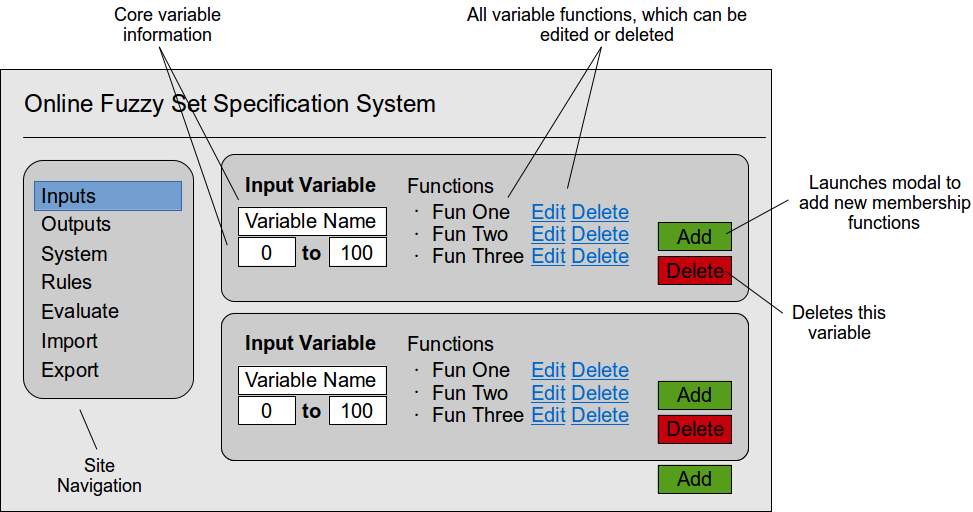
\includegraphics[width=0.9\textwidth]{images/firstItInputs}
\end{center}
\vspace{-2mm}
\caption{The first iteration of the design of the input creation page}
\label{fig:design-firstIterationInputs}
\vspace{-1mm}
\end{figure}
\noindent 
The first iteration of the input creation page listed the navigation to the left hand side of the page, as this is a standard positioning for navigation, and the users would, most likely, be accustomed to this. \ \\
\ \\
The separation of different tasks to different sections of the website is very important for the construction of a fuzzy system, as there are many individual elements, and a lack of separation of these would cause a great deal of confusion for the user, as there would be a huge number of elements on the screen at one time.\ \\
\ \\
The design displays the core information of the variable on the far left (including name and range), as this is where the user's eye would fall first. The next set of information (the functions contained within the variable), are displayed further to the right, as the user would look to here after reading the initial information. The users have the option to edit or delete any function that they have created, granting them complete freedom over the system and everything they do within it. They also have the option to add a new membership function (which is a green button, to represent creation, which brings up a modal window to be used to construct the membership function), or delete the current variable (which is a red button, to represent destruction). \ \\
\ \\
This design uses long horizontal representations of the variables, so a large number of them can be on the screen at the same time, as they take up little vertical space. This means the users can view many of their variables at the same time, and make edits as necessary. Colour is used sparingly throughout the page, so that it can be used effectively for highlighting important information or elements, so they are easily visible to the user.

\begin{figure}[ht!]	
\begin{center}
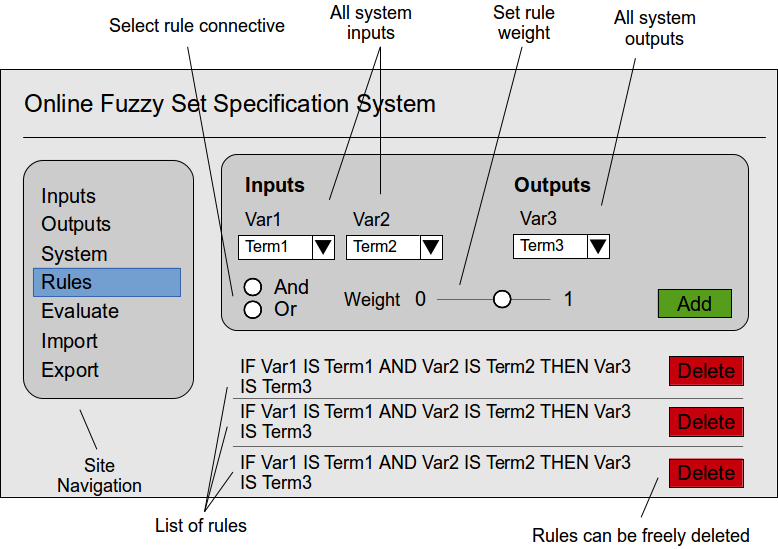
\includegraphics[width=0.9\textwidth]{images/firstItRules}
\end{center}
\vspace{-5mm}	
\caption{The first iteration of the design of the rule creation page}
\label{fig:design-firstIterationRules}
\end{figure}
\noindent 
The rule creation page also follows a horizontal theme, which is especially effective for the rules, as there could potentially be a long list of them. The creation of the rules, and their displaying, are two clearly distinct segments to the page, which means there is no confusion between the two, and the process remains a simple one.\ \\
\ \\
In keeping with the standards of the previous page, the ``Add'' button is coloured green, to represent creation, and the ``Delete'' buttons present by each rule is coloured red, to represent destruction. These clear colour separations are useful to the user, as they do not even need to read a button to gain an understanding of what it will do, and they can be more careful to not make mistakes.\ \\
\ \\
As can be seen, the navigation and header of the rule creation page are the same as those on the input creation page, which promotes a consistent style amongst the pages, and helps to remind the user they are still within the same system, even if they are completing a different task. 





\subsubsection{Second Iteration}

\begin{figure}[ht!]
\begin{center}
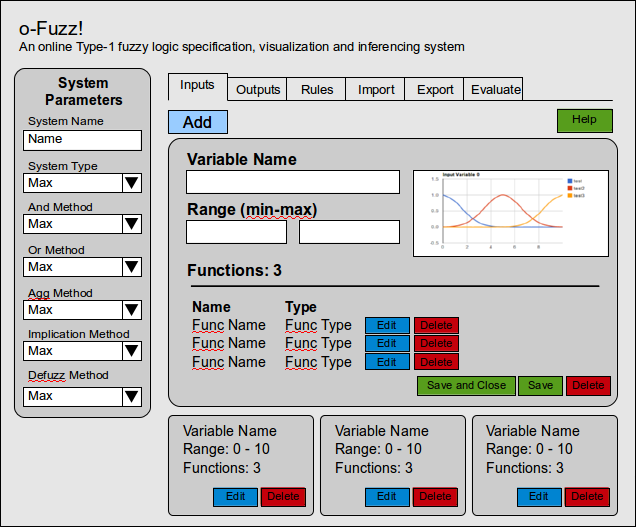
\includegraphics[width=0.8\textwidth]{images/secondItInputs}
\end{center}
\caption{The second iteration of the design of the input creation page}
\label{fig:design-secondIterationInputs}
\end{figure}
\noindent

\noindent 
The second iteration of the input creation page design includes many improvements over the first iteration. Specifically, this second iteration dealt with the issues the first iteration presented, and had well known and well documented usability heuristics and design principles applied to it, to ensure optimality. \ \\
\ \\
One of the largest changes to the design was the re-working of the navigation to be entirely tabular, and to replace the old navigation area with system wide parameters segment. This tabbing helps to split the different tasks of the system in an intuitive manner, as most users are familiar with the concept of tabs, due to their popularity within internet browsers \cite{huang2010parallel}. The system wide parameters are now displayed in place of the old navigation, which means they can be changed, regardless of the tab the user is on. This is especially convenient when the user comes to evaluate the system, as it makes tuning much quicker, and all permutations of parameters can be evaluated with ease.\ \\
\ \\
The overall structure and displaying of the variables has also been drastically changed in this second iteration of design. The reason for this was that, whilst the old design promoted a large number of variables on the screen at any one time, this would severely increase the cognitive load on the user, and they could quickly become confused.\ \\
\ \\
The new design works by having expandable and collapsible variables. When in the collapsed view, the variable takes up a much smaller space, displaying only key information, and in the expanded view, all of the information of the variable is present (like in the previous design). The ideal number of elements on a page is 7$\pm$2 \cite{miller1956magical}, which can easily be exceeded with these new collapsed variables. However, the reason this design works, is because when the variable is collapsed, the user feels like it is completed, and they no longer need to concern themselves with it. So whilst this new design may look more cluttered, it significantly helps to reduce the cognitive load of the user, as they can create a variable, and then essentially forget about it.\ \\
\ \\
To fit with the consistency of the other pages, the buttons for the editing and deletion of membership functions have also been changed. The edit button is now blue, which is the system wide colour for editing, and the delete buttons are now red, the system wide colour for deletion. This keeps the website consistent, and makes the functionality of these buttons easily identifiable.\ \\
\ \\
A graphical representation of each variable is now also displayed in the expanded view, allowing the user to quickly interpret how their system is progressing, and whether it looks as they expected. This is a very powerful tool, as users will be able to spot errors much sooner than if this were not present.\ \\
\ \\
Some other smaller changes include the moving of the ``Add'' button from the bottom right of the page, to the top left. The reason for this is that, in the first iteration of design, the add button would constantly move down the page as variables were added, and a moving button can be frustrating and confusing for some users. Another change is the addition of a short name for the software, with a longer tag-line underneath this, at the top of the page. This shortened title allows for users to refer to system with ease, allowing them to search for help for the system if necessary, and simply discuss the system with other potential users. The longer tag-line allows for a brief description of the system, so the user knows whether it will be able to accomplish the tasks they have set out to achieve.


\begin{figure}[ht!]
\begin{center}
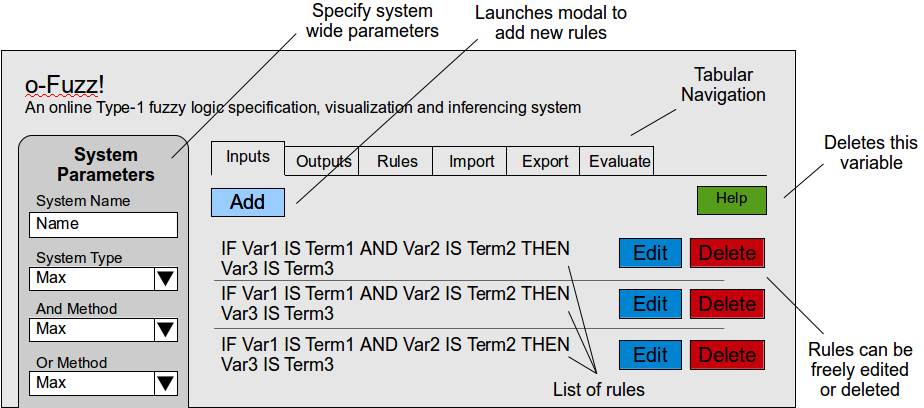
\includegraphics[width=0.8\textwidth]{images/secondItRules}
\end{center}
\caption{The second iteration of the design of the rule creation page}
\label{fig:design-secondIterationRules}
\end{figure}
\noindent 
The rules creation page also received heavy changes in the second iteration. The first of these was the inclusion of certain features that were not present in the first design, but were necessary for the functioning of the program. For instance, the ability to edit rules once they had been created, the ability to create negated terms (for instance, ``If food is \textit{not} good'') and the addition of the help button to the page.\ \\
\ \\
However, the biggest change is the removal of the ability to create rules on this initial page. Instead, as with the creation of membership functions, this has been moved into a separate window that is launched when the user clicked the ``Add'' button. This reduces the clutter on the page, and means the rule creation functionality is only accessed when the user requires it (helping to reduce cognitive load on the user).\ \\
\ \\
In addition, an extra feature was included in the form of a rule table that could be displayed if the user was using a system with two inputs, and one output (a relatively common set up for a fuzzy system). If this were the case, the table would be displayed, mapping the inputs to the outputs, in an intuitive graphical manner, an example of which can be seen in figure \ref{fig:ruleTable}.

\begin{figure}[ht!]
\begin{center}
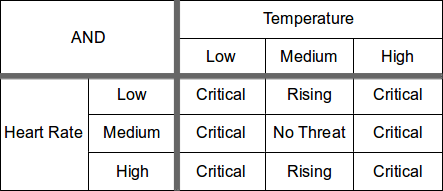
\includegraphics[width=0.575\textwidth]{images/ruletable}
\end{center}
\vspace{-4mm}
\caption{An example of a rule table that would be displayed if the user had two inputs (heart rate and temperature) and a single output (urgency)}
\label{fig:ruleTable}
\end{figure}

\subsubsection{Heuristic Evaluation of Second Iteration}\ \\
The new design also went through a heuristic evaluation \cite{nielsen1990heuristic}, using the Usability Heuristics laid out by Jakob Nielson \cite{nielsen2005ten}, and the Golden Rules for Design, laid out by Ben Shneiderman \cite{shneiderman2005designing}. Both of whom are extremely well known and very influential in the field of Human Computer Interaction, and their heuristics define some of the most basic, but most important properties a user interface should possess. 

\begin{enumerate}
\item Visibility of system status/Offering of informative feedback\\

It is important that the users of a system are always updated as to what is happening within the system. This will be implemented through the use of JavaScript alert messages to alert the user to any errors they have made, or any important changes they have taken place.

\item User control and freedom/Support internal locus of control\\
The user should be in full control of their experience of the system at all times, and thus a fluid and flexible navigation system is important. This is the purpose of the tabular layout of the website, as the user is free to travel to whichever pages they wish, in whichever order. More details on the navigation of the system can be found in section \ref{subsec:nav}.

\item Consistency and standards/Strive for consistency\\
A good interface should also be consistent in it's design, and follow platform standards. As you can see from the design of the input creator and the rule creator pages, the tabular layout is consistent throughout the website, and colours such as blue, green, and red have clearly defined purposes, which stay consistent throughout the as well.

\item Error prevention/ Help users recognize, diagnose, and recover from errors\\
Unfortunately, with a system that is entirely dictated by user input, it is very difficult to prevent the user from making errors. However, measures will be put in place to ensure these errors do not affect the system. For instance, there is no way to enforce the user of a system to enter a number, but an informative error message will be displayed, telling the user this is not valid, and what should be done to rectify the issue (and, of course, not accepting the value into the system).

\item Recognition rather than recall/Reduce short-term memory load\\
As mentioned multiple times already, the system is designed to reduce cognitive load on the user as much as possible. This is done by reducing the number of elements on the page at any one time, and by using modal windows for the creation of new membership functions and rules, so their creation and their display are distinct.

\item Aesthetic and minimalist design\\
To reduce any possible distractions for the user, the system is designed in a minimalistic fashion, using colour very sparingly, and sticking to neutral shades for background elements. The only colour used in the system is on the graphs drawn, and on the important buttons the user will be pressing. These buttons are essentially colour coded so the user is aware of their functionality, without even having to read them. Further to this, the use of modal windows to essentially hide functionality greatly helps to reduce clutter on the pages of the website, giving it a much cleaner look.

\item Help and documentation\\
Due to the goal of being as easy as use as possible, the system is to be designed with a dedicated help system, built in. The advantage of this is that the user is able to access help without having to leave the application itself, meaning a minimised distraction time. Help is accessed via the large green help button present on every page, which is easily visible, and provides concise and helpful information for the user.

\end{enumerate}
\noindent 
As the final stage of the heuristic evaluation process, the ``sins'' of New Media Design \cite{golombisky2013white} were also evaluated, to ensure an optimal design had been produced. The second iteration of design has taken these sins into account and has avoided those that were appropriate. Specifically, the website features no bulky borders, a generous use of margins, left alignment of elements (as opposed to centring), and an avoidance of a busy background, opting instead for a very simple white background. All of the aforementioned design choices could have easily caused distractions for the user, and damaged their enjoyment of the system.

\subsection{Navigation/Control Flow Design}	
\label{subsec:nav}	
As of the second iteration of the design, the website has six main sections, enumerated below;
\begin{enumerate}
\item Inputs;
The page used to construct input variables of the system
\item Outputs;
The page used to construct output variables of the system
\item Rules;
The page used to construct rules of the system
\item Evaluate;
The page used to evaluate the system
\item Import;
The page used to import files into the system
\item Export;
The page used to export file from the system
\end{enumerate}
\noindent 
The generally \emph{expected} path for a user of the system to take, would be to launch the system to the input creation screen (the landing page), on which they would spent some time constructing their input variables. They would then move to the output variables, construct those, and then move onto the rules, and construct those. At this point, the path splits between evaluating the system, exporting it for later, or a mixture of the two. \ \\
\ \\
Due to the ability to import files, an entirely new path is also available throughout this process, in which the user begins by importing a file, and then either editing it, or going straight to evaluating it.\ \\
\ \\
The expected path through the system (beginning at the inputs page, as this is the landing page of the website), is represented in figure \ref{fig:pathThrough}

\begin{figure}[ht!]
\begin{center}
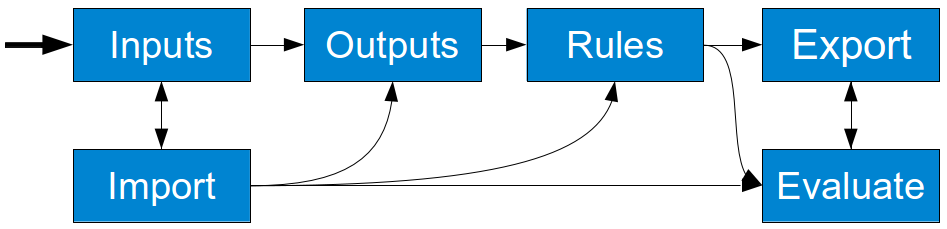
\includegraphics[width=0.75\textwidth]{images/genericPathOne}
\end{center}
\caption{Expected path a user would take through the system}
\label{fig:pathThrough}
\end{figure}
\noindent 
Of course, whilst the general path through the system has been determined, this is not the only path through the system, and there is no guarantee that the user will follow this path. In fact, the user has the freedom to traverse the system in any path they please, as shown in figure \ref{fig:webThrough}. This is important for promoting freedom and a sense of control within the system. The user is free to decide how they wish to travel through the system, and this means they are free to traverse forward or backward through the system to make any alterations, or fix any mistakes they may have made.

\begin{figure}[ht!]
\begin{center}
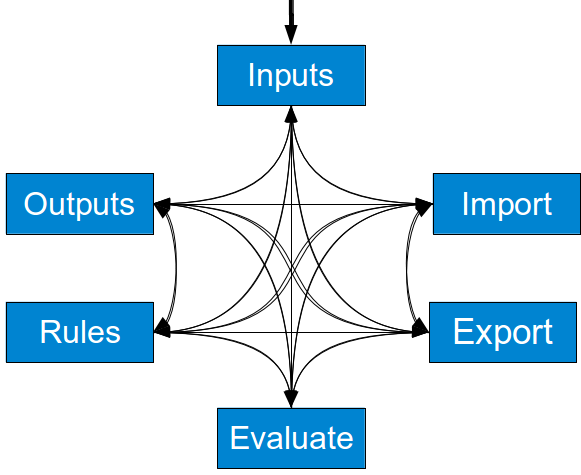
\includegraphics[width=0.6\textwidth]{images/web}
\end{center}
\caption{Possible paths through the system}
\label{fig:webThrough}
\end{figure}

\subsection{Internal Design}
The user interface of a system is a huge part of the design process, and is extremely important, as this will be how the user will actually be interacting with it. However, this is not the only part of the system that requires designing; as the internal workings of the system also require a lot of thought. \ \\
\ \\
For this project, a web-interface was to be used to interact with a back end that could deal the processing of a fuzzy logic system. By this point in the project's development, the software's implementation decisions had been made (which are detailed in section \ref{sec:kid}), and the decision of the back end to be used was the FuzzyToolkitUoN R Package, using the R-Shiny service, to interact between the front end and back end. The diagram in figure \ref{fig:architectureDiagram} shows how the interaction between these two systems is handled.

\begin{figure}[ht!]
\begin{center}
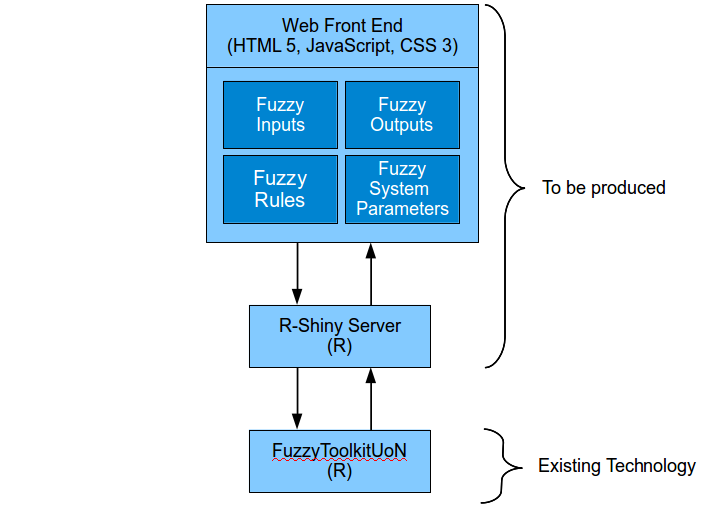
\includegraphics[width=0.9\textwidth]{images/architecture}
\end{center}
\caption{Interaction between the back end and front end of the system}
\label{fig:architectureDiagram}
\end{figure}

\noindent
As you can see, the web front end will be constructed using HTML 5, JavaScript, and CSS 3, and will allow for the creation and specification of fuzzy inputs, outputs, rules, and system parameters. Once a system has been specified, and the user chooses to evaluate the system, the information of the system is passed to the R-Shiny server. This then takes all the form elements from the web front end, extracts their values, and constructs a FIS file, within R. This can then have functions from the FuzzyToolkitUoN package applied to it, and the results of these functions can then be passed back to the web front end, for display to the user.

\section{Software Implementation}

{\color{red} 
Implementation containing a comprehensive description of the implementation of your software, including the language(s) and platform chosen, problems encountered, any changes made to the design as a result of the implementation, etc
}

\section{Evaluation of the Project}
% as part of jakon nielsons usability engineering life cycle 
\cite{nielsen1992usability}
% i did some user evaluation


% mention how someone obviously said the errors were friendly

\subsection{Functionality Testing}
%	{\color{red}
%		check the software fits the functional requirements. Tests that look at the functionality of the system, including the individual components and the communication between the different parts. Give a list of tests, and the results of each of these tests, to ensure each functional requirement has been met.
%	}
\subsection{User Feedback Testing}
%	{\color{red}
%		Comparisons against other software, and checking against non-functional requirements. General explanation about the tests, and the participants, and what we are looking for (non functional, usability, accessibility). talk about using disseration to do fuz coursework. ``Considering I wrote both FTU and oFuzz, i found oFuzz much easier to use. Having the fuz coursework gave me a unique experience to test using both systems, as a user, instead of as the developer.''
		
%		{\color{blue}
%		An important part of evaluating the usability and accessibility of my system was to have real world users attempt to actual use not only my system, but similar systems, so that they could make comparative comments. In order to do this, I set up several sessions in which I would invite users of various skills levels, both in terms of computers, and fuzzy logic, to complete a list of tasks using all three software systems, after which I would ask them to give their feedback and opinions on all the systems. The three software systems that were evaluated were: my project, the MATLAB fuzzy toolbox, and FuzzyToolkitUoN, within the standard R environment.\ \\
%		\ \\
%		I split the participants into four main categories, based on their skill levels in terms of using computers, and knowledge of fuzzy logic. There were a total of 23 participants in these studies, and the distribution of skill levels is displayed in figure \ref{fig-skills}. The reason for this split was so that these distinctive groups could be evaluated individually, and their specific requirements could be observed. For instance, a participant skilled in computers, but not in fuzzy logic, would not struggle in navigating a system, but could potentially struggle understanding some of the fuzzy terminology.
		
%		\begin{figure}[ht!]
%		\begin{center}
%		\begin{tabular}{cc|cc}
%			& &\multicolumn{2}{c}{Computer Skill} \\
%			& & Low & High \\
%			\hline 
%		    \multirow{2}{2cm}{Fuzzy Logic Skill}  & Low & 7 & 5  \\
%		     &  High                                    & 3 & 8  \\
%		     \hline
%		     \\
%		     \multicolumn{3}{r}{\textbf{Total}} & 23\\
%		\end{tabular}
%		\end{center}
%		\vspace{-5mm}
%		\caption{Distribution of participant skill levels}
%		\label{fig-skills}
%		\vspace{-2mm}
%		\end{figure}
%		\noindent 
%		The task assigned to the participants was designed to use as much of the different systems as possible, but focused mainly on cross-compatible parts of the systems, so they could be easily compared. The test itself was to construct the fuzzy tipper example, using service and food as inputs, to produce a number for the tip to leave (the full set of instructions can be found in appendix \ref{app-userEval}). 
%		}
%	}
	\subsubsection{Evaluation of FuzzyToolkitUoN}
%		{\color{red}
%			Good things, bad things, statistics to back this up, talk about non funcs, and mention each type of user
%		}
	\subsubsection{Evaluation of MATLAB Fuzzy Toolbox} 	
%		{\color{red}
%			As above, but comparisons with above. specificaly mention that MATLAB has milliions of windows to open which make it very confusing!!!		
%		}
	\subsubsection{Evaluation of My Project}	
%		{\color{red}
%			As above, but comparison with above and above above
%		}
	\subsubsection{Summary}	
%		{\color{red}
%			Overall results and comparative statistics. 
%			{\color{blue}
%			The main two factors that were observed whilst the participants were completing the tasks were the speed at which they could do so, and the ease. Generally a faster completion meant either a high level of understanding, or an easier piece of software to use. The data collected strongly suggests that completion of the task using FuzzyToolkitUoN was the most difficult, which after speaking to the participants was the result of a poor user interface, and a very steep learning curve (especially for those of a novice computer skill level). The graph in figure \ref{fig:times} shows box plots of the completion times of each of the tasks, for each of the different groups. Each of these plots shows that FuzzyToolkitUoN was the most time consuming task to complete (taking on average {\color{red} 100 seconds}), and that the graphical systems were much easier to use (with MATLAB on average, taking {\color{red} 40 \%} less time, and my new system taking {\color{red} 10 \%} less time than that).
			
%			\begin{figure}[ht!]
%			\begin{center}
%			some graph yo
%			\end{center}
%			\vspace{-5mm}
%			\caption{Time taken to complete the tasks in the different software systems}
%			\label{fig:times}
%			\vspace{-2mm}
%			\end{figure}
			
%			Whilst the time taken to complete the tasks was a strong indicator of the success of the software system, it was also important to ask the participants which system they enjoyed using the most. The results for this were conclusive, which 100\% of participants (across all categories) claiming FuzzyToolkitUoN was the piece of software they enjoyed using the least. {\color{red} This is because...}. The piece of software that the participants enjoyed using the most was {\color{red} x \%} in favour of my produced software, over MATLAB (and the majority of those that said they preferred MATLAB said so as they were already very familiar with MATLAB). The results for most favoured,  software system can be seen in figure \ref{fig:mostleast}, organised by category of participant. {\color{red} The main reasons for an attraction to MATLAB were... and o-fuzz}
			
%			\begin{figure}[ht!]
%			\begin{center}
%			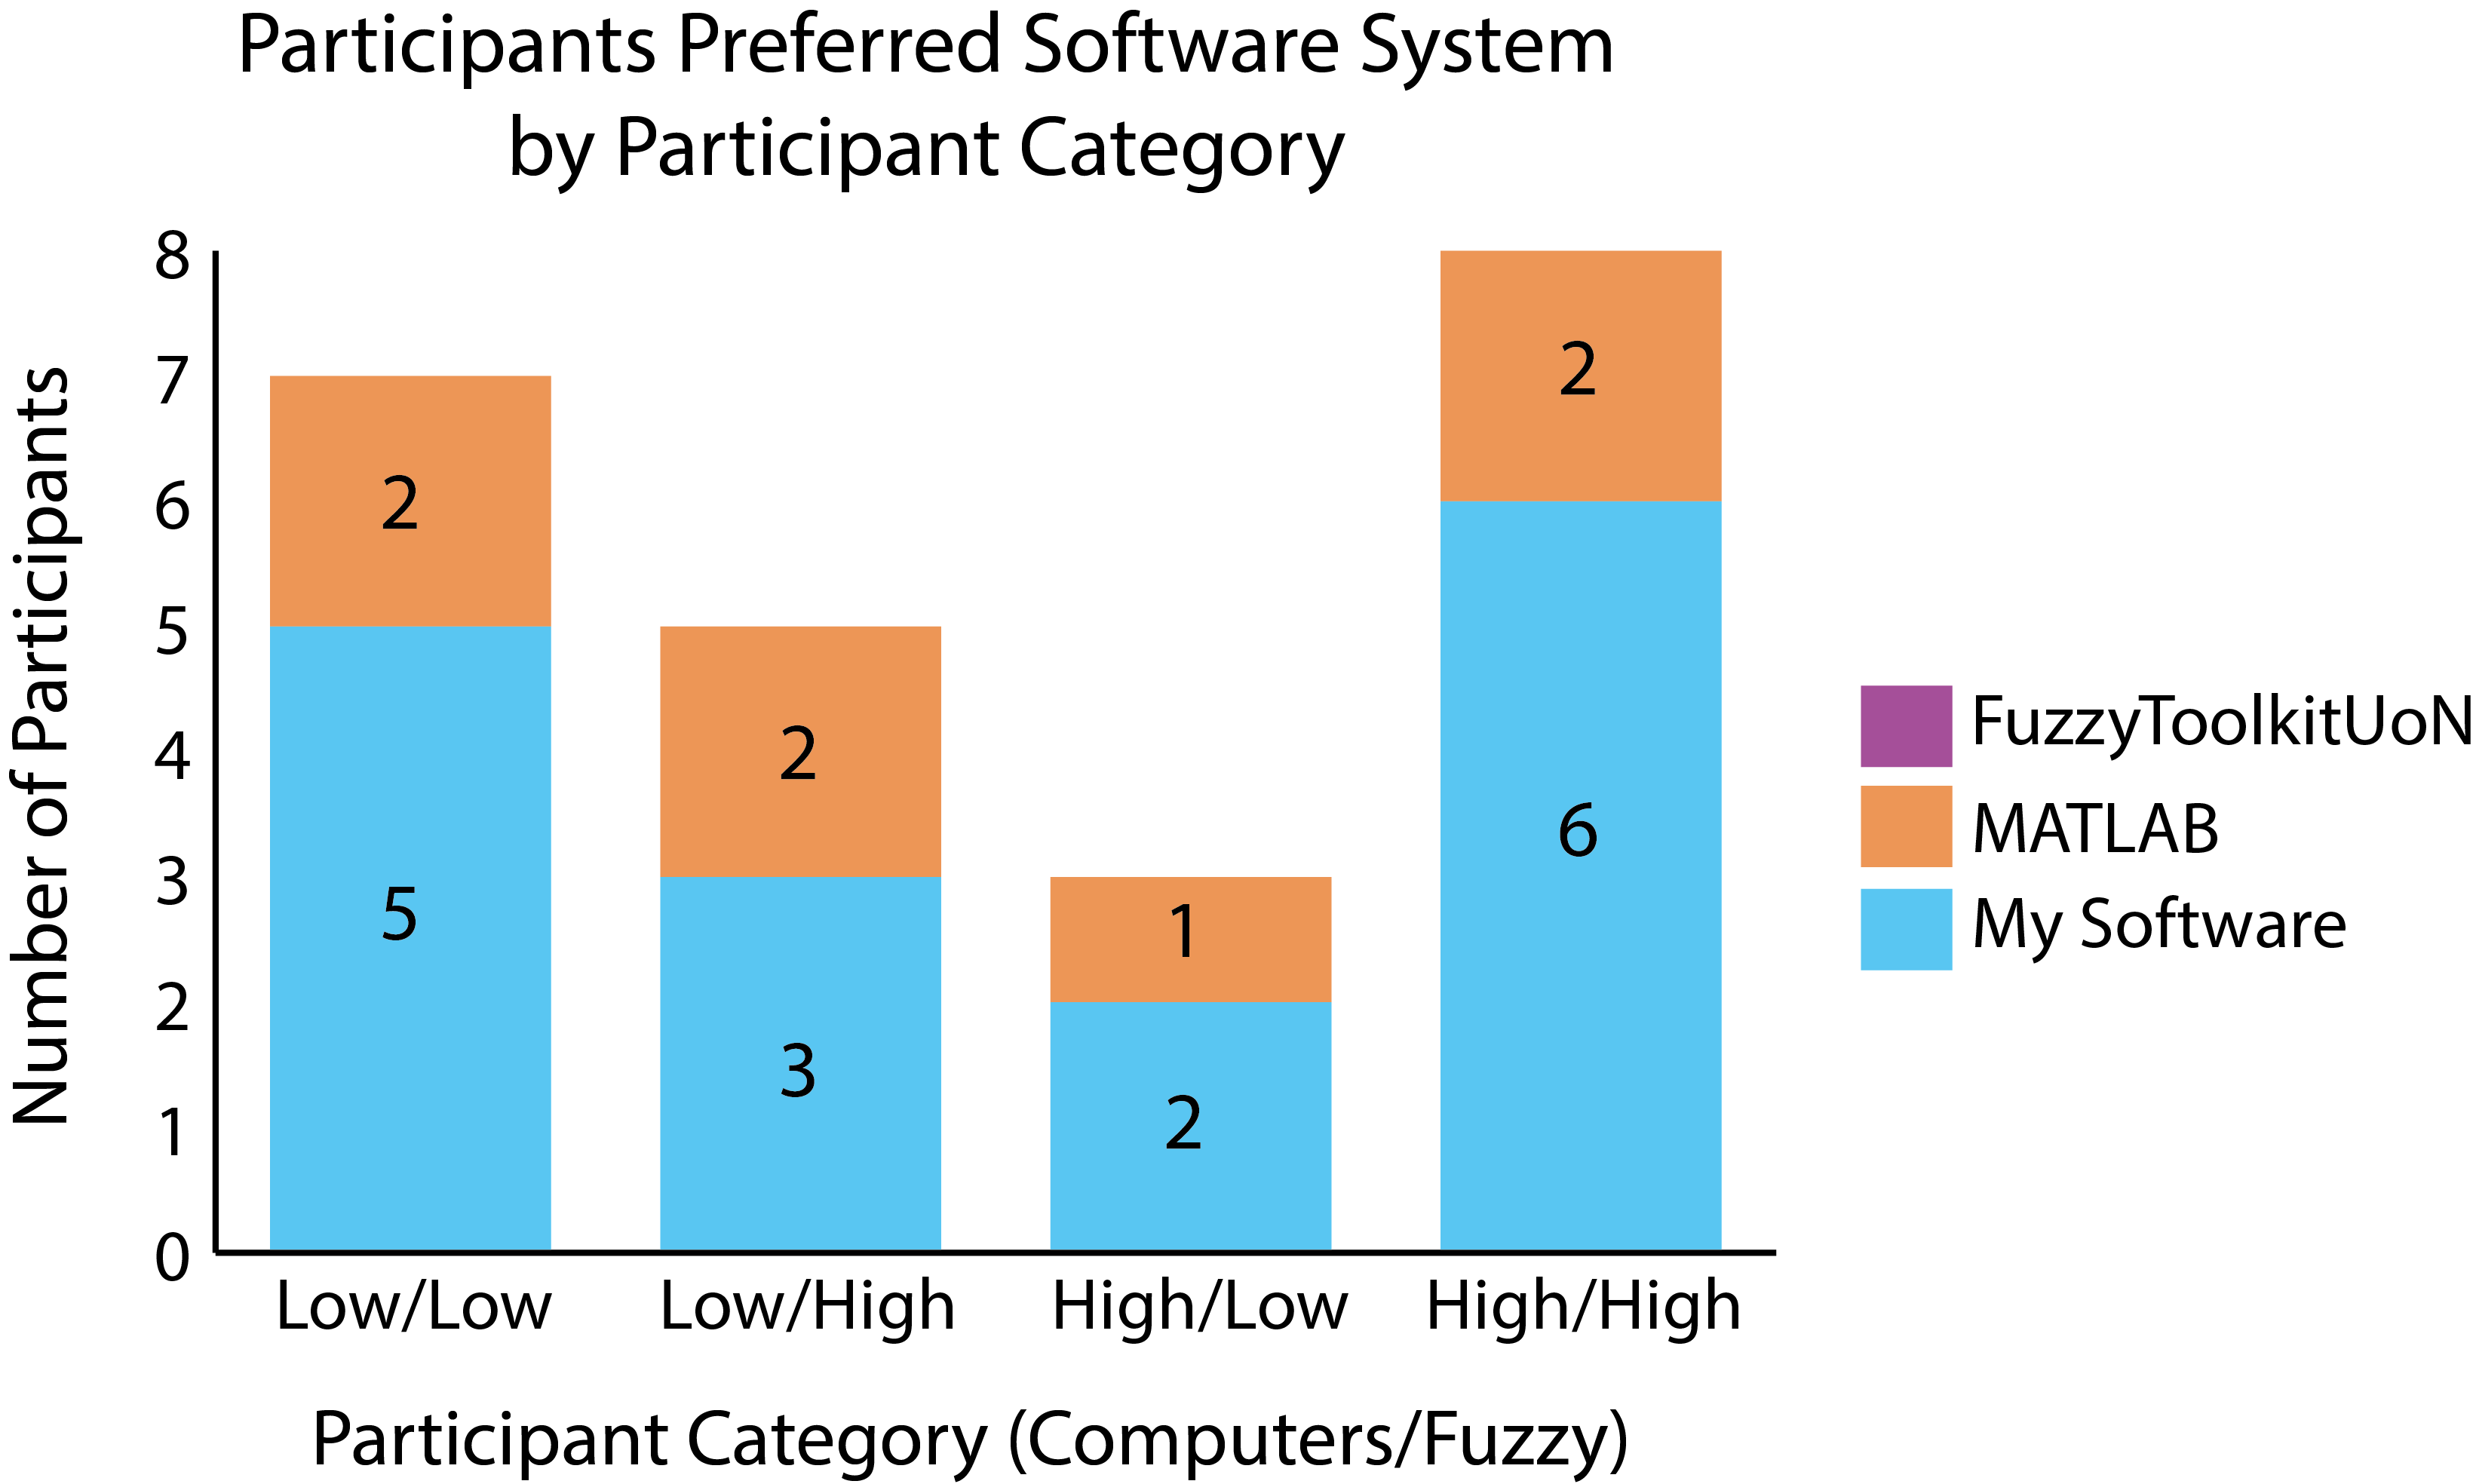
\includegraphics[width=0.8\textwidth]{images/graphsSmall.png}
%			\end{center}
%			\vspace{-5mm}
%			\caption{Favoured/Least Favoured software system, by participant category}
%			\label{fig:mostleast}
%			\vspace{-2mm}
%			\end{figure}
%			}
%		}		


\subsection{Successes and Limitations of the Project}
%{\color{red} 
%Explain what went well with the project, what didn't go so well, and what could be done better for next time (with concrete goals). issues with FTU as the backend (some options in params disabled because they don't work in FTU - not my fault!).

%}

\section{Further Work}
{\color{red}further... work?}

\subsection{Type-2 Fuzzy Logic}
\label{sec:type2}

\section{Summary \& Personal Evaluation}
Personally, I feel as thought the project was a success, as it solved the two main issues it was conceived to solve, it met all the functional and non-functional requirements set out, and user feedback was almost entirely positive. Another reason that I believe the project was successful is that I have used the software myself, and found it a pleasurable experience. During the life time of the project, I enrolled in a module at the University of Nottingham known as \emph{Fuzzy Sets and Fuzzy Systems}\cite{uon2014fuz}. In this module, I was required to use FuzzyToolkitUoN to construct a system that would advise a doctor on how urgently a patient should be sent to the hospital, based on their heart rate and temperature. However, I found FuzzyToolkitUoN cumbersome to use (which, considering I helped to produce it, shows how poor of a piece of software it is), and instead used the prototype version of my dissertation software. This greatly sped up the process of completing this work, and gave me a unique experience to test my system as an end user.\ \\
\ \\
This was the largest project that I had ever worked on by myself, but I felt as though I rose to the challenge, and employed several clever methods in order to help manage my time, and the work to be completed (such as a Kanban Board, and the use of a Gantt Chart). I did not always stick to the time scale set out by my Gantt chart, due to other work, and commitments, but the combination of the Gantt chart to track the ``big-picture'', and the Kanban board to track individual features made the management of the project much simpler.\ \\
\ \\
One of the areas I feel as though was weaker within the project, was the research segment, or more specifically, research into software that could be used. Whilst multiple examples were evaluated against one another, this ``research'' was more of a superficial overview of the software, instead of an in-depth analysis. As a result of this, half way through the implementation, many issues began to arise with the tools chosen. The most prominent of these was the inability to properly construct dynamic user interfaces and have these interface with R-Shiny, and the numerous bugs and issues discovered whilst using FuzzyToolkitUoN. I also feel as though the testing process could have been much more rigorous, as numerous issues arose throughout the life time of the software development, and solving them was often time consuming, and cumbersome.\ \\
\ \\
If I could work on this project again, from the beginning, there are several changes that I would make. The first of these would be a more rigorous evaluation of the tools that would be used, so that the major issues that arose with this project would not have done so. The other major change would be to implement Unit Testing and Test Driven Development from the start of the project, so that the code quality could be ensured throughout, and bugs easily identified. This includes integration, and regression testing, which would have made the addition of new features, and any extensions to the software, much simpler and easier to debug.

\null
\vfill
\begin{flushright}
	\begin{tabular}{r|l}
		Words in text	& 4,717 \\
	\end{tabular}
	\ \\
	\ \\
	\begin{tabular}{cc}
		\multicolumn{2}{r}{Calculated with the TeXCount web service}\\
		\multicolumn{2}{r}{\url{http://app.uio.no/ifi/texcount/online.php}}
	\end{tabular}
\end{flushright}

%
%
% Bibliography
%
%

\newpage
\pagestyle{biblio}
\bibliographystyle{plain}

\bibliography{bib}


%
%
%  Appendix 
% 
%
\newpage
\setcounter{page}{1}
\pagestyle{appendix}
\appendix
\section{User Evaluation Test Instructions}
\label{app-userEval}
The purpose of this test is to construct the fuzzy logic tipper example, in three different software systems, so that the strengths and weaknesses of each of these systems can be identified. The tipper example is a simple fuzzy system that uses food quality (rated from 0 to 10) and service quality (rated from 0 to 10) as inputs, to determine how much of a tip should be left (between 0 and 30 percent). \ \\
\ \\
Please follow the instructions below, and do not hesitate to ask for help if you are stuck, this is an evaluation of the user interface, and not of you. After each step, please explain your thought process, and how you found the task.

\begin{enumerate}
\item (\textbf{FuzzyToolkitUoN only}) Create a new \textbf{Fuzzy Inference System}
\item Add a new \textbf{input variable}, called \textbf{Service}, with range \textbf{0} to \textbf{10}
\item Add the following \textbf{membership functions} to the \textbf{Service} variable
	\begin{enumerate}
	\item A \textbf{Gaussian} function, named \textbf{Poor}, with parameters:\\
	\begin{tabular}{ll}
	Sigma 	& 1.5 \\
	Mean	& 0   \\
	Height	& 1   \\
	\end{tabular}
	\item A \textbf{Gaussian} function, named \textbf{Good}, with parameters:\\
	\begin{tabular}{ll}
	Sigma 	& 1.5 \\
	Mean	& 5   \\
	Height	& 1   \\
	\end{tabular}	
	\item A \textbf{Gaussian} function, named \textbf{Excellent}, with parameters:\\
	\begin{tabular}{ll}
	Sigma 	& 1.5 \\
	Mean	& 10   \\
	Height	& 1   \\
	\end{tabular}	
	\end{enumerate}
\item Add a new \textbf{input variable}, called \textbf{Food}, with range \textbf{0} to \textbf{10}	
\item Add the following \textbf{membership functions} to the \textbf{Food} variable
	\begin{enumerate}
	\item A \textbf{Trapezoidal} function, named \textbf{Rancid}, with parameters:\\
	\begin{tabular}{ll}
	Left Foot 		& 0		\\
	Left Shoulder 	& 0		\\
	Right Shoulder 	& 1		\\
	Right Foot 		& 3		\\
	Height			& 1   	\\
	\end{tabular}
	\item A \textbf{Trapezoidal} function, named \textbf{Delicious}, with parameters:\\
	\begin{tabular}{ll}
	Left Foot 		& 7		\\
	Left Shoulder 	& 9		\\
	Right Shoulder 	& 10	\\
	Right Foot 		& 10	\\
	Height			& 1   	\\
	\end{tabular}		
	\end{enumerate}
\newpage 
\item Add a new \textbf{output variable}, called \textbf{Tip}, with range \textbf{0} to \textbf{30}	
\item Add the following \textbf{membership functions} to the \textbf{Tip} variable
	\begin{enumerate}
	\item A \textbf{Triangular} function, named \textbf{Cheap}, with parameters:\\
	\begin{tabular}{ll}
	Left  			& 0		\\
	Mean 			& 5		\\
	Right 			& 10		\\
	Height			& 1   	\\
	\end{tabular}
	\item A \textbf{Triangular} function, named \textbf{Average}, with parameters:\\
	\begin{tabular}{ll}
	Left  			& 10		\\
	Mean 			& 15		\\
	Right 			& 20		\\
	Height			& 1   	\\
	\end{tabular}	
	\item A \textbf{Triangular} function, named \textbf{Generous}, with parameters:\\
	\begin{tabular}{ll}
	Left  			& 20		\\
	Mean 			& 25		\\
	Right 			& 30		\\
	Height			& 1   	\\
	\end{tabular}			
	\end{enumerate}	
\item Add the following \textbf{rules} to the system
	\begin{enumerate}
	\item IF Service is Poor OR Food is Rancid, Then Tip is Cheap (Weight 1)
	\item IF Service is Average, Then Tip is Average (Weight 1)
	\item IF Service is Excellent OR Food is Delicious, Then Tip is Generous (Weight 1)
	\end{enumerate}
\item (\textbf{FuzzyToolkitUoN, and o-Fuzz only}) Please evaluate the following values:
	\begin{enumerate}
	\item Service score of 0, Food score of 0
	\item Service score of 10, Food score of 10
	\end{enumerate}
\item Please change the \textbf{defuzzification method}	of the system to \textbf{Bisector}
\item \textbf{Save} the inference system as a file to your hard drive
\item Now, read that same file back into the system
\end{enumerate}

\newpage
\section{Table of Results of User Evaluation}
\label{app-torous}



\begin{center}
\begin{tabular}{cccc}
\hline
\textbf{Group} 	& \textbf{\# of Members} & \textbf{Fuzzy Logic Skill} & \textbf{Computer Skill} \\
\hline
1				& 7 						 & Low			& Low		\\	
2				& 5  						 & Low			& High		\\
3				& 3 						 & High			& Low 		\\
4				& 8 						 & High 		& High		\\
\hline
\end{tabular}
\end{center}

\noindent 
This table lists the time taken (in Minutes) for each participant to complete each task of the expirement. Task 1 was to follow the instruction list using FuzzyToolkitUoN, Task 2 was to follow the instruction list using the MATLAB Fuzzy Toolbox and Task 3 was to follow the instruction list using the new project created in this report. It also details the participants favourite, and least favourite software, of the three (OF standing for O-Fuzz, this project, FTU standing for FuzzyToolkitUoN, and M standing for MATLAB's fuzzy toolbox).\ \\
\begin{changemargin}{-1cm}{-1cm}
\begin{tabular}{ccccccc}
\hline
Participant	&	Group	&	Task 1	&	Task 2	&	Task 3	&	Most Liked Software	&	Least Liked Software 	\\
\hline
1			&	1		&	53		&	21		&	14		&	OF					&	FTU						\\	
2			&	1		&	45		&	23		&	15		&	OF					&	FTU						\\
3			&	1		&	61		&	34		&	20		&	OF					&	FTU						\\	
4			&	1		&	70		&	36		&	21		&	M					&	FTU						\\	
5			&	1		&	63		&	31		&	15		&	OF					&	FTU						\\		
6			&	1		&	53		&	23		&	13		&	M					&	FTU						\\	
7			&	1		&	54		&	26		&	16		&	OF					&	FTU						\\	
8			&	2		&	35		&	13		&	9		&	OF					&	FTU						\\		
9			&	2		&	25		&	14		&	8		&	M					&	FTU						\\	
10			&	2		&	27		&	15		&	10		&	OF					&	FTU						\\			
11			&	2		&	26		&	11		&	11		&	OF					&	FTU						\\		
12			&	2		&	31		&	14		&	10		&	M					&	FTU						\\		
13			&	3		&	33		&	16		&	9		&	M					&	FTU						\\	
14			&	3		&	30		&	16		&	10		&	OF					&	FTU						\\			
15			&	3		&	40		&	33		&	13		&	OF					&	FTU						\\			
16			&	4		&	14		&	11		&	4 		&	OF					&	FTU						\\		
17			&	4		&	28		&	12		&	6 		&	OF					&	FTU						\\			
18			&	4		&	20		&	10		&	6 		&	M					&	FTU						\\	
19			&	4		&	21		&	12		&	5 		&	OF					&	FTU						\\			
20			&	4		&	12		&	13		&	6 		&	FTU					&	M 						\\			
21			&	4		&	25		&	10		&	4 		&	OF					&	FTU						\\		
22			&	4 		&	18		&	14		&	5 		&	OF					&	FTU						\\
23			&	4 		&	16		&	11		&	5 		&	M					&	FTU						\\
\hline
\end{tabular}			
\end{changemargin}
\newpage 
\section{Complete Test Listing}
\label{app-ctl}
\begin{longtable}{p{5cm}|p{6cm}|p{3cm}}
\hline 
\textbf{Test} & \textbf{Expected Results} & \textbf{Actual Results} \\
\hline 
Users will be able to create Gaussian membership functions 
& There will be an option to specify a Gaussian membership function
& As expected \\ 
\hline
  \multicolumn{3}{c}{
  \fbox{ \raisebox{-\totalheight}{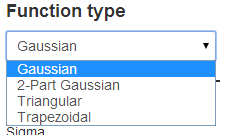
\includegraphics[width=0.3\textwidth]{images/test1.png}} }}\\
  \multicolumn{3}{l}{ }     \\\hline
Users will be able to create 2-Part Gaussian membership functions 
& There will be an option to specify a 2-Part Gaussian membership function
& As expected \\ 
\hline
  \multicolumn{3}{c}{
  \fbox{ \raisebox{-\totalheight}{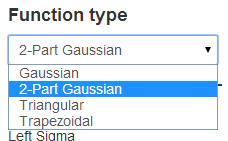
\includegraphics[width=0.3\textwidth]{images/test1-a.png}} }}\\
 \multicolumn{3}{l}{ }     \\\hline
Users will be able to create Triangular membership functions 
&There will be an option to specify specify a Triangular membership function
& As expected \\ 
\hline
  \multicolumn{3}{c}{
  \fbox{ \raisebox{-\totalheight}{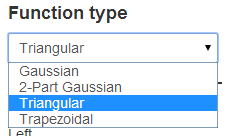
\includegraphics[width=0.3\textwidth]{images/test1-b.png}} }}\\
 \multicolumn{3}{l}{ }     \\\hline
Users will be able to create Trapezoidal membership functions 
& There will be an option to specify a Trapezoidal membership function
& As expected \\ 
\hline
  \multicolumn{3}{c}{
  \fbox{ \raisebox{-\totalheight}{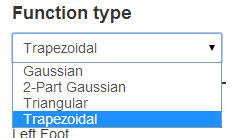
\includegraphics[width=0.3\textwidth]{images/test1-c.png}} }}\\
 \multicolumn{3}{l}{ }     \\








\hline Users will be able to add membership functions to variables 

& There will be a button to add membership functions to variables 

& As expected \\ 
  \hline
 \multicolumn{3}{c}{ \raisebox{-\totalheight}{
\includegraphics[width=0.5\textwidth]{images/test2.png}} }\\ 
 \multicolumn{3}{l}{ }     \\\hline

Users will be able edit membership function names 
& There will be a ``function name'' parameter box 
& As Expected \\ 
  \hline
 \multicolumn{3}{c}{
 \fbox{ \raisebox{-\totalheight}{
\includegraphics[width=0.3\textwidth]{images/test4.png}} }}\\ 
 \multicolumn{3}{l}{ }     \\\hline

Users will be able edit membership function parameters 
& There will be input boxes to specify function parameters 
& As Expected \\ 
  \hline
 \multicolumn{3}{c}{\fbox{ \raisebox{-\totalheight}{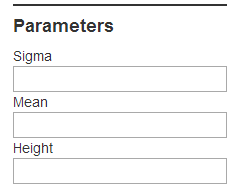
\includegraphics[width=0.3\textwidth]{images/test5.png}} }}\\ 
 \multicolumn{3}{l}{ }     \\\hline

Users will be able to delete membership functions from variables 
&  Each function will have a delete button
& As Expected \\ 
  \hline
 \multicolumn{3}{c}{ \raisebox{-\totalheight}{
\includegraphics[width=0.5\textwidth]{images/test3.png}} }\\ 
 \multicolumn{3}{l}{ }     \\\hline

Users will be able to access help on how to create membership functions 
& There will be a show help button, that when pressed, will display an explanation of the window & 
As Expected\\ 
  \hline
 \multicolumn{3}{c}{ \raisebox{-\totalheight}{
\includegraphics[width=0.3\textwidth]{images/test6.png}} }\\ 
 \multicolumn{3}{l}{ }     \\\hline

Users will be able to see a plot of their membership functions 
&  A plot of the membership function will be displayed after all parameters have been given
& As Expected\\ 
  \hline
 \multicolumn{3}{c}{ \raisebox{-\totalheight}{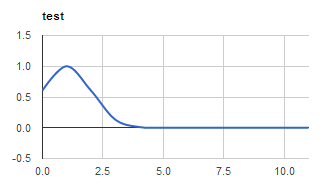
\includegraphics[width=0.4\textwidth]{images/test7.png}} }\\ 
 \multicolumn{3}{l}{ }     \\\hline

Users will be able to create input linguistic variables 
& There will be an ``inputs'' tab, with an ``Add New Variable'' button
& As Expected \\ 
  \hline
 \multicolumn{3}{c}{
 \fbox{ \raisebox{-\totalheight}{
\includegraphics[width=0.5\textwidth]{images/test8.png}} }}\\ 
 \multicolumn{3}{l}{ }     \\\hline

Users will be able to create output linguistic variables& There will be an ``outputs'' tab, with an ``Add New Variable'' button
& As Expected \\  
  \hline
 \multicolumn{3}{c}{\fbox{ \raisebox{-\totalheight}{
\includegraphics[width=0.5\textwidth]{images/test9.png}} }}\\ 
 \multicolumn{3}{l}{ }     \\\hline

Users will be able to edit the range of linguistic variables 
& There will be input boxes for both minimum and maximum range
& As Expected \\ 
  \hline
 \multicolumn{3}{c}{ \raisebox{-\totalheight}{
\includegraphics[width=0.3\textwidth]{images/test11.png}} }\\ 
 \multicolumn{3}{l}{ }     \\\hline

Users will be able to delete variables & There will be a button that deletes variables & As Expected \\ 
  \hline
 \multicolumn{3}{c}{ \raisebox{-\totalheight}{
\includegraphics[width=0.5\textwidth]{images/test12.png}} }\\ 
 \multicolumn{3}{l}{ }     \\\hline

Users will be able to rename variables & There will be an input box to change the name of a variable & As Expected \\ 
  \hline
 \multicolumn{3}{c}{ \raisebox{-\totalheight}{
\includegraphics[width=0.3\textwidth]{images/test13.png}} }\\ 
 \multicolumn{3}{l}{ }     \\\hline

Users will be able to access help on how to create variables &  There will be a show help button, that when pressed, will display an explanation of the page  & As Expected  \\ 
  \hline
 \multicolumn{3}{c}{\fbox{ \raisebox{-\totalheight}{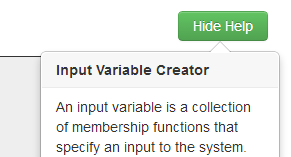
\includegraphics[width=0.3\textwidth]{images/test14.png}} }}\\ 
 \multicolumn{3}{l}{ }     \\\hline

Users will be able to create rules for the system & There will be an ``Add New Rule'' button on the Rules page & As Expected \\ 
  \hline
 \multicolumn{3}{c}{\fbox{ \raisebox{-\totalheight}{
\includegraphics[width=0.45\textwidth]{images/test15.png}} }}\\ 
 \multicolumn{3}{l}{ }     \\\hline

Users will be able to specify rule terms & There will be dropdown boxes for each variable in the system, that users can select terms from & As Expected \\ 
  \hline
 \multicolumn{3}{c}{ \raisebox{-\totalheight}{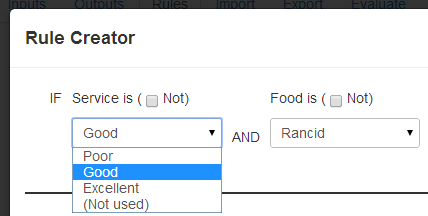
\includegraphics[width=0.4\textwidth]{images/test16.png}} }\\ 
 \multicolumn{3}{l}{ }     \\\hline

Users will be able to negate certain terms in a rule & There will be a checkbox above each term, symbolising negation & As Expected \\ 
  \hline
 \multicolumn{3}{c}{\fbox{ \raisebox{-\totalheight}{
\includegraphics[width=0.25\textwidth]{images/test17.png}} }}\\ 
 \multicolumn{3}{l}{ }     \\\hline

Users will be able to change the weight of a rule & There will be a slider, and input box, to change the rule weight & As Expected \\ 
  \hline
 \multicolumn{3}{c}{\fbox{ \raisebox{-\totalheight}{
\includegraphics[width=0.4\textwidth]{images/test18.png}} }}\\ 
 \multicolumn{3}{l}{ }     \\\hline

Users will be able to specify the connective to be used in the rule & There will be a set of radio buttons to toggle between connectives & As Expected  \\ 
  \hline
 \multicolumn{3}{c}{\fbox{ \raisebox{-\totalheight}{
\includegraphics[width=0.2\textwidth]{images/test19.png}} }}\\ 
 \multicolumn{3}{l}{ }     \\\hline

Users will be able to edit any previously constructed rules & There will be an edit button aside each constructed rule & As Expected \\ 
  \hline
 \multicolumn{3}{c}{\fbox{ \raisebox{-\totalheight}{
\includegraphics[width=0.45\textwidth]{images/test20.png}} }}\\ 
 \multicolumn{3}{l}{ }     \\\hline

Users will be able to delete any previously constructed rules & There will be a  delete button aside each constructed rule & As Expected \\ 
  \hline
 \multicolumn{3}{c}{\fbox{ \raisebox{-\totalheight}{
\includegraphics[width=0.45\textwidth]{images/test21.png}} }}\\ 
 \multicolumn{3}{l}{ }     \\\hline

Users can access help on how to create rules &  There will be a show help button, that when pressed, will display an explanation of the window & As Expected \\ 
  \hline
 \multicolumn{3}{c}{\fbox{ \raisebox{-\totalheight}{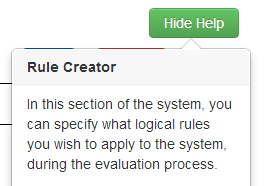
\includegraphics[width=0.3\textwidth]{images/test22.png}} }}\\ 
 \multicolumn{3}{l}{ }     \\\hline

Users will be able to edit the name of the system & There will be an input box to edit the name of the system & As Expected \\ 
  \hline
 \multicolumn{3}{c}{ \raisebox{-\totalheight}{
\includegraphics[width=0.3\textwidth]{images/test23.png}} }\\ 
 \multicolumn{3}{l}{ }     \\\hline

Users will be able to edit the type of evaluation to use &  There will be an input box to edit the type of the system & As Expected \\ 
  \hline
 \multicolumn{3}{c}{ \raisebox{-\totalheight}{
\includegraphics[width=0.3\textwidth]{images/test24.png}} }\\ 
 \multicolumn{3}{l}{ }     \\\hline

Users will be able to edit the ``and'' method to use &  There will be an input box to edit the ``and'' method of the system & As Expected  \\ 
  \hline
 \multicolumn{3}{c}{ \raisebox{-\totalheight}{
\includegraphics[width=0.3\textwidth]{images/test25.png}} }\\ 
 \multicolumn{3}{l}{ }     \\\hline

Users will be able to edit the ``or'' method to use & There will be an input box to edit the ``or'' method of the system & As Expected  \\ 
  \hline
 \multicolumn{3}{c}{ \raisebox{-\totalheight}{
\includegraphics[width=0.3\textwidth]{images/test26.png}} }\\ 
 \multicolumn{3}{l}{ }     \\\hline

Users will be able to edit the aggregation method to use & There will be an input box to edit the aggregation method of the system &  As Expected \\ 
  \hline
 \multicolumn{3}{c}{ \raisebox{-\totalheight}{
\includegraphics[width=0.3\textwidth]{images/test27.png}} }\\ 
 \multicolumn{3}{l}{ }     \\\hline

Users will be able to edit the implication method to use & There will be an input box to edit the implication method of the system & As Expected  \\ 
  \hline
 \multicolumn{3}{c}{ \raisebox{-\totalheight}{
\includegraphics[width=0.3\textwidth]{images/test28.png}} }\\ 
 \multicolumn{3}{l}{ }     \\\hline

Users will be able to edit the defuzzification method to use & There will be an input box to edit the defuzzification method of the system &  As Expected \\ 
  \hline
 \multicolumn{3}{c}{ \raisebox{-\totalheight}{
\includegraphics[width=0.3\textwidth]{images/test29.png}} }\\ 
 \multicolumn{3}{l}{ }     \\\hline

Users will be able to access help on what affect these changes make &  There will be a show help button, that when pressed, will display an explanation of the parameters & As Expected  \\ 
  \hline
 \multicolumn{3}{c}{ \raisebox{-\totalheight}{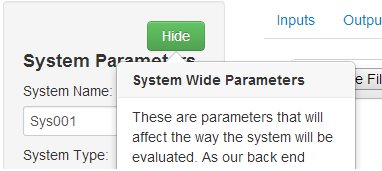
\includegraphics[width=0.4\textwidth]{images/test30.png}} }\\ 
 \multicolumn{3}{l}{ }     \\\hline

Users will be able to export their system as a MATLAB .fis file & On the export page, there will be an option to download a MATLAB .fis file & As Expected  \\ 
  \hline
 \multicolumn{3}{c}{ \raisebox{-\totalheight}{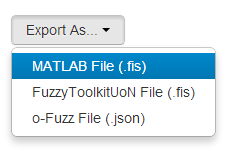
\includegraphics[width=0.3\textwidth]{images/test31.png}} }\\ 
 \multicolumn{3}{l}{ }     \\\hline

Users will be able to export their system as a FuzzyToolkitUoN .fis file & On the export page, there will be an option to download a FuzzyToolkitUoN .fis file & As Expected \\ 
  \hline
 \multicolumn{3}{c}{ \raisebox{-\totalheight}{
\includegraphics[width=0.3\textwidth]{images/test32.png}} }\\ 
 \multicolumn{3}{l}{ }     \\\hline

Users will be able to export their system as a JSON file & On the export page, there will be an option to download a JSON file &  As Expected \\ 
  \hline
 \multicolumn{3}{c}{ \raisebox{-\totalheight}{
\includegraphics[width=0.3\textwidth]{images/test33.png}} }\\ 
 \multicolumn{3}{l}{ }     \\\hline

Users can access help on how to export files and what is supported &  There will be a show help button, that when pressed, will display an explanation of the window & As Expected \\ 
  \hline
 \multicolumn{3}{c}{\fbox{ \raisebox{-\totalheight}{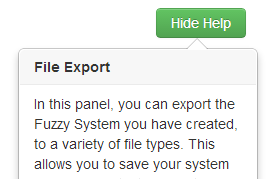
\includegraphics[width=0.3\textwidth]{images/test34.png}} }}\\ 
 \multicolumn{3}{l}{ }     \\\hline

Users will be able to import a MATLAB .fis file & Importing of MATLAB .fis files will be supported within the system & As Expected \\ 
  \hline
 \multicolumn{3}{c}{ \raisebox{-\totalheight}{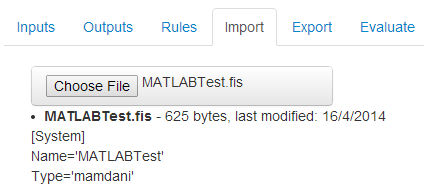
\includegraphics[width=0.5\textwidth]{images/test36.png}} }\\ 
 \multicolumn{3}{l}{ }     \\\hline

Users will be able to import a FuzzyToolkitUoN .fis file &  Importing of FuzzyToolkitUoN .fis files will be supported within the system & As Expected \\ 
  \hline
 \multicolumn{3}{c}{ \raisebox{-\totalheight}{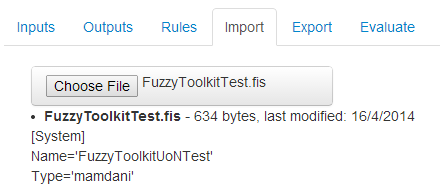
\includegraphics[width=0.5\textwidth]{images/test37.png}} }\\ 
 \multicolumn{3}{l}{ }     \\\hline

Users will be able to import a JSON file &  Importing of JSON files will be supported within the system & As Expected \\ 
  \hline
 \multicolumn{3}{c}{ \raisebox{-\totalheight}{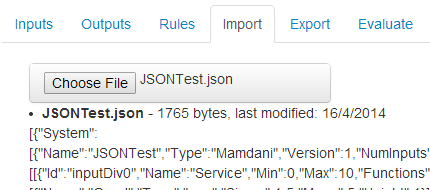
\includegraphics[width=0.5\textwidth]{images/test38.png}} }\\ 
 \multicolumn{3}{l}{ }     \\\hline

Users can access help on how to import files and what is supported &  There will be a show help button, that when pressed, will display an explanation of the window & As Expected \\ 
  \hline
 \multicolumn{3}{c}{\fbox{ \raisebox{-\totalheight}{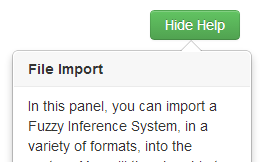
\includegraphics[width=0.3\textwidth]{images/test35.png}} }}\\ 
 \multicolumn{3}{l}{ }     \\\hline

Users can provide a value for each input, and receive the output value & An input box for each system input will be displayed, and an appropriate output displayed for each combination of input value provided  & As Expected \\ 
  \hline
 \multicolumn{3}{c}{\fbox{ \raisebox{-\totalheight}{\includegraphics[width=0.4\textwidth]{images/test39.png}} }}\\ 
 \multicolumn{3}{l}{ }     \\\hline

Users can access help on how the evaluation process works &  There will be a show help button, that when pressed, will display an explanation of the window & As Expected \\
  \hline
 \multicolumn{3}{c}{ \raisebox{-\totalheight}{\includegraphics[width=0.3\textwidth]{images/test40.png}} }\\ 
 \multicolumn{3}{l}{ }     \\

  \end{longtable}


%
%
% Qed
%
%

\end{document}








	